\documentclass[tikz]{standalone}
\usepackage[compat=1.1.0]{tikz-feynman}

\begin{document}

% gluon fusion
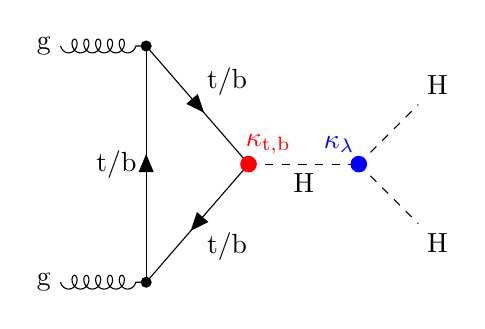
\begin{tikzpicture}
  \begin{feynman}
    \vertex at (0,3) (top) {g};
    \vertex at (1.3,3) (cup);
    \vertex at (0,1.5) (mid);
    \vertex at (0,0) (bot) {g};
    \vertex at (1.3,0) (cdo);
    \vertex at (2.6,1.5) (kappa);
    \vertex at (4, 1.5) (h);
    \vertex at (5, 2.5) (h1) {H};
    \vertex at (5, 0.5) (h2) {H};
    
    \diagram* [horizontal=mid to h] {
      (top) -- [gluon] (cup),
      (bot) -- [gluon] (cdo),
      (cup) -- [fermion, edge label = t/b] (kappa) -- [fermion, edge label = t/b] (cdo) -- [fermion, edge label = t/b] (cup),
      (kappa) -- [scalar, edge label = H, swap] (h),
      (h) -- [scalar] (h1),
      (h) -- [scalar] (h2),
    };
  \end{feynman}

  \fill[red] (kappa) circle (3pt);
  \node[red] at ($(kappa) + (0.25,0.25)$) {$\kappa_{\mathrm{t},\mathrm{b}}$};
  \fill[blue] (h) circle (3pt);
  \node[blue] at ($(h) + (-0.25,0.25)$) {$\kappa_{\lambda}$};
  \fill[black] (cup) circle (2pt);
  \fill[black] (cdo) circle (2pt);
\end{tikzpicture}

\end{document}
